\documentclass[handout]{beamer}

\usepackage{fontspec} 
% \usepackage{lsp-makros}
\useoutertheme{lsp}

\usepackage{lsptitle}

\def\two@digits#1{\ifnum#1<10 0\fi\number#1}
\def\mytoday{\two@digits{\number\day}.\two@digits{\number\month}.\number\year}


\usepackage{xspace,multicol}
\newcommand{\latex}{\LaTeX\xspace}
\usepackage{tikz}


\newcounter{lastpagemainpart}
\footnotesep0pt
\renewcommand{\footnoterule}{}
\usefootnotetemplate{
  \noindent
  \insertfootnotemark\insertfootnotetext}

\let\beamerfn=\footnote
\renewcommand{\footnote}[1]{%
\let\oldfnsize=\footnotesize%
\let\footnotesize=\tiny%
\beamerfn<\thebeamerpauses->{#1}%
\let\footnotesize=\oldfnsize}


\date{\today}

\usepackage{eurosym}  
 
\renewcommand{\centerline}[1]{\hfill#1\hfill\hfill\mbox{}}


\title{Aufbau eines Zyklus für Offenes Publizieren}
% \institute{FU Berlin}
\author[LangSci]{Sebastian Nordhoff @langscipress, HU Berlin}



\begin{document}
\lspbeamertitle


% \section{Language Science Press}
% \frame{
% \frametitle{Language Science Press}
% %   \includegraphics[height=.2\textheight]{./path/to/graphicsfile}
%   \begin{itemize}
%     \item linguistische Monographien und Sammelbände als CC-BY
%     \item  aktiv seit 2014 (FU Berlin), seit 2017 HU Berlin
%     \item  Ziel: maximale Offenheit des Publikationsprozesses
%   \end{itemize}
% }

\section{Open X}

\frame{
\frametitle{Offenheit: Open X}
   \Huge         \mbox{Open Access}
   \LARGE        \mbox{Open Source}
    \huge        \mbox{Open Data }
    \large       \mbox{Open Hardware}
    \LARGE       \mbox{Open Government}
    \Large       \mbox{Open Educational Resources}
    \huge        \mbox{Open GLAM     }
    \large       \mbox{Open Labs}
}


\frame{ 
\frametitle{Open Source}

\includegraphics[width=2.5cm]{starofficelogo.png}~$\Longrightarrow$~%

\includegraphics[width=4cm]{openofficelogo.png}~$\Longrightarrow$~%

\includegraphics[width=3cm]{libreofficelogo.png}
\\[2em]
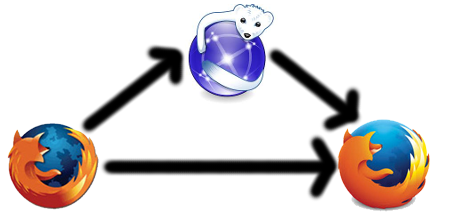
\includegraphics[width=5cm]{firefoxiceweasel.png}
} 

 
    
\frame{
\frametitle{Open Data \\(hier: Open Transport Data)}

\begin{columns}
  \begin{column}{7cm}
    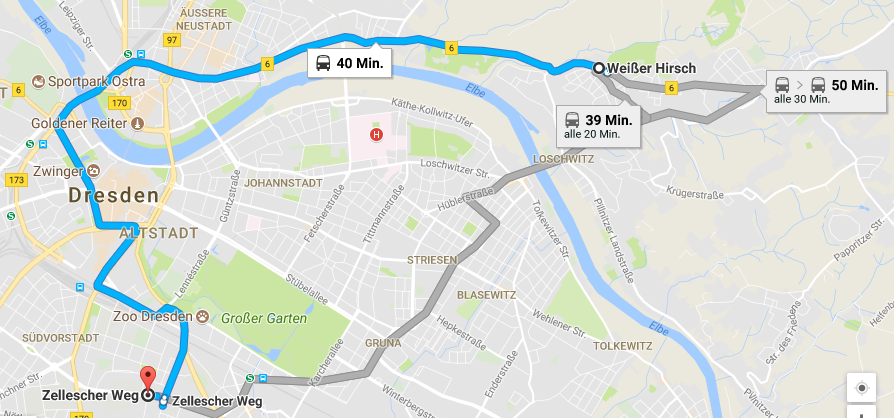
\includegraphics[width=7.5cm]{zellescherweg.png}
  \end{column}
  \begin{column}{3cm}
    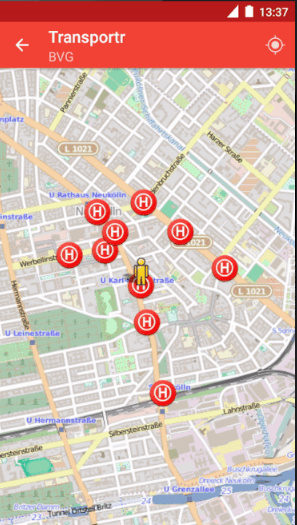
\includegraphics[height=.85\textheight]{transportr.png}
  \end{column}
\end{columns}

}

   
\frame{
\frametitle{Und Open Access? }
\begin{itemize}
 \item ``Read-only''-Ausprägung von Offenheit
 \item Hauptanwendungsfall der Nachnutzung: Text Mining
 \begin{itemize}
  \item explorativ
 \end{itemize}
 \item Im allgemeinen wenig Interesse, das Werk an sich zu verändern
 \begin{itemize}
  \item anders als in Open Source, Open Hardware, Open GLAM, OER
  \item dort Modifikation ein Hauptantriebsfaktor
 \end{itemize}
 \item weiterer Anwendungsfall: Neuzusammenstellung (Arrangement) z.B. auf Science Open
\end{itemize}
}
 
\section{Technische Anforderungen} 
 \frame{
\frametitle{\raggedright Technische Anforderungen\\	 für mehr Offenheit und\\ Veränderbarkeit}

\begin{tabular}{l||l} 
Produzentenseite & Rezipientenseite\\
\hline
 \\
 \parbox{5cm}{
 \begin{itemize}
  \item Versionierungssystem
  \begin{itemize}
   \item commits, branches, forks, merges, issues
  \end{itemize}
  \item frei zugänglich
  \item BYOB (build your own book)
 \end{itemize}
}&
\parbox{5cm}{
 \begin{itemize}
 \item kollaborative Annotationssoftware
  \begin{itemize}
   \item online
   \item frei zugänglich
   \item Verankerung am Text
  \end{itemize}
 \end{itemize}
}\\
\hline
\\

\includegraphics[height=1cm]{github.png}&
\includegraphics[height=1cm]{paperhive.png} \\
\end{tabular}
}
   
    
\frame{
\frametitle{Github: Issue-Tracker}
    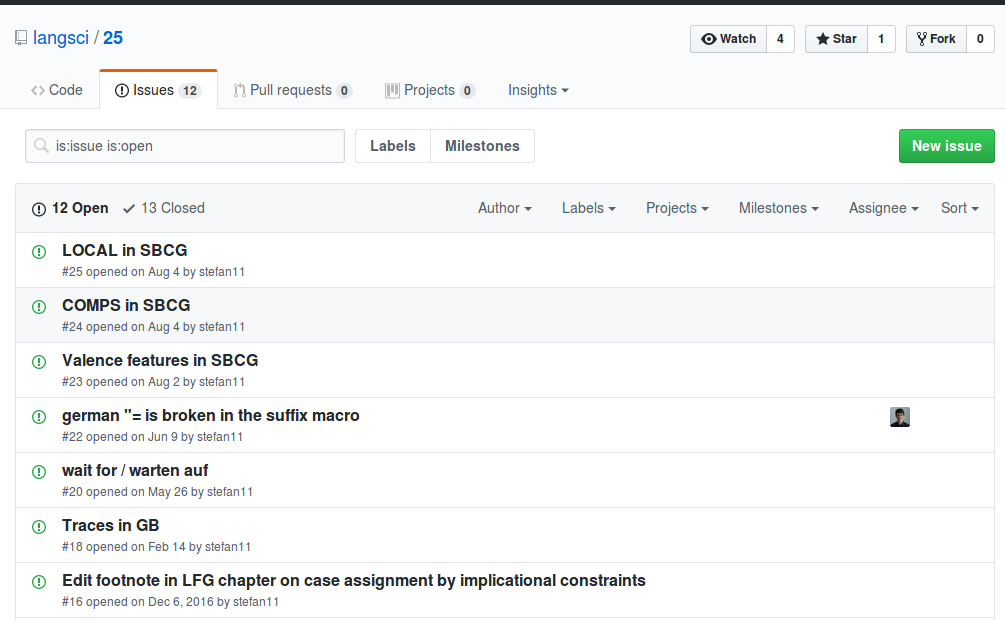
\includegraphics[height=\textheight]{issues.png}	
}
    
\frame{
\frametitle{Versionierungssystem: Git(Hub)}
\begin{columns}
  \begin{column}{2.5cm}
    \begin{itemize}
   \item commits
   \item branches
   \item forks
   \item merges
   \item releases\\\medskip 
   \item issues
  \end{itemize}
  \end{column}
  \begin{column}{8cm}
    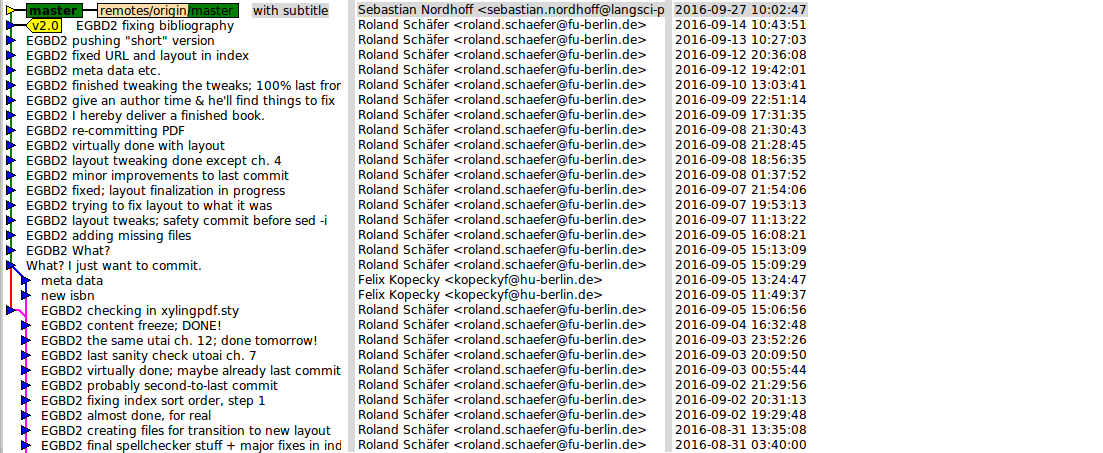
\includegraphics[height=\textheight]{gittree.png}
  \end{column}
\end{columns}
}



% \frame{ 
% \frametitle{Rezipientenseite}
% \begin{itemize}
%  \item ``User-Generated Improvement''
%  \begin{itemize}
%   \item Open Review
%   \item Community Proofreading
%   \item Post-Publication Comments
%  \end{itemize}
% 
% \end{itemize}
% 
% 
% }

\frame{ 
\frametitle{\mbox{Rezipientenseite} \mbox{Open Review}}
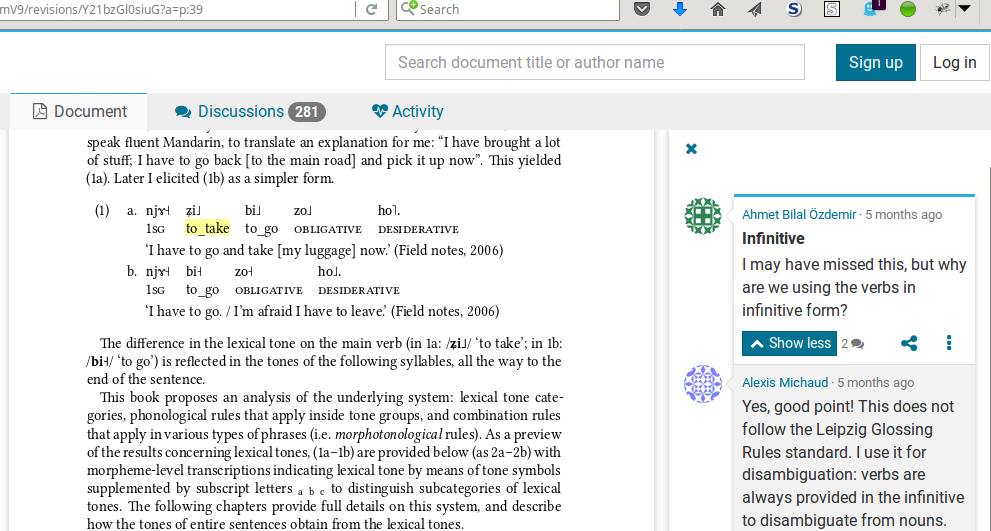
\includegraphics[width=\textwidth]{openreview.png}
}

\frame{ 
\frametitle{\mbox{Rezipientenseite}  \mbox{Community Proofreading}}
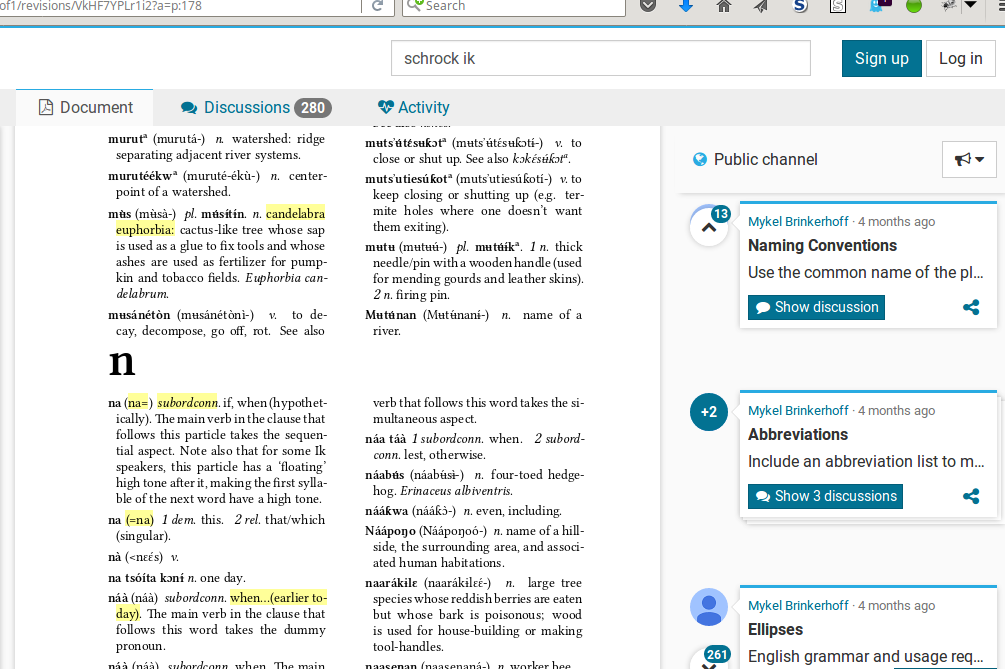
\includegraphics[width=\textwidth]{communityproofreading.png}
}

\frame{ 
\frametitle{\mbox{Rezipientenseite} \mbox{Post Publication Comments}}
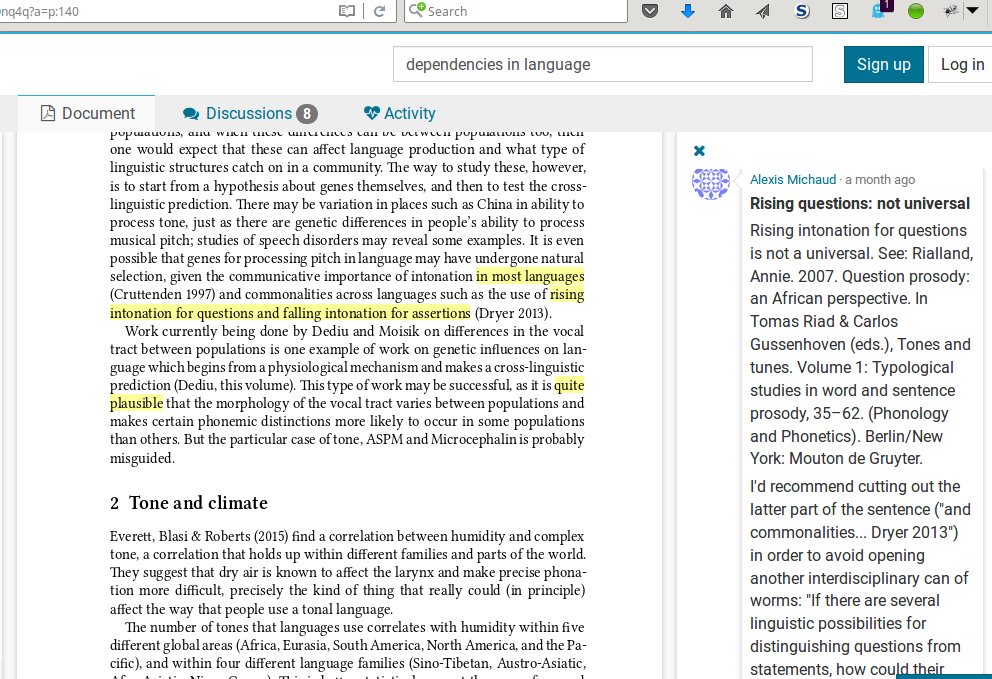
\includegraphics[width=\textwidth]{postpublicationcomments.png}
}

\section{Desiderata}

\frame{
\frametitle{Was fehlt: die Ehe}
\begin{itemize}
 \item Verbindung von Rezipientenseite und Autorenseite
 \item Verbindung von Online-Annotation und Issue-Tracking
 \item Verbindung von Paperhive und GitHub
\end{itemize}
  \hspace*{4cm}  
\includegraphics[height=.7\textheight]{marriage.png}
}

 
\frame{
\frametitle{Prototypefund:\\ docloop-OER}
\parbox{.35\textwidth}{

\includegraphics[width=.35\textwidth]{prototypefund.png}\\
~~~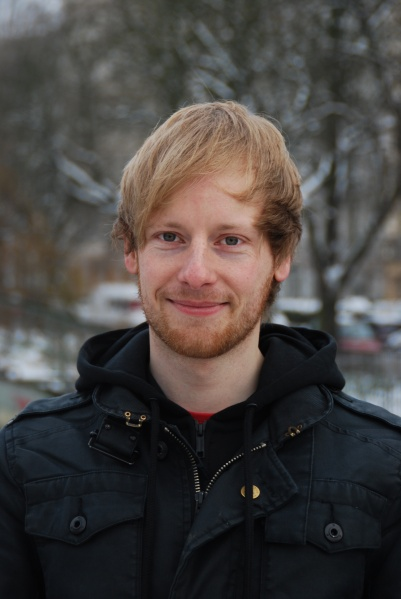
\includegraphics[width=.3\textwidth]{pittrich.jpg}
}
\parbox{7cm}{
\begin{itemize}
 \item Das BMBF fördert über den Prototypefund das Projekt docLoop-OER mit 30.000 EUR
 \item Zurückspielen von Leserkommentaren in das Issue-Tracking-System auf Autorenseite
 \item Für OER, aber im Prinzip auf beliebige Inhalte übertragbar
 \item Start: 1.9.2017\\ \url{rhotep.github.io/docLoop/}
\end{itemize}
}


}

 
 
 
% \frame{
% \frametitle{Frametitle3}
% %   \includegraphics[height=.2\textheight]{./path/to/graphicsfile}
%   \begin{itemize}
%     \item  
%     \item 
%   \end{itemize}
% }

%\setcounter{framenumber}{\thelastpagemainpart}
\end{document}